\section{Meditation on the Trinity}

Before he had begun publishing his major works, \textbf{Rene Guenon} engaged in an extended correspondence with the writer \textbf{Noëlle Maurice-Denis}, daughter of the painter \textbf{Maurice Denis}. In a letter from 1919, he explained his life project to Noëlle, which was to develop a ``common understanding" ``between various traditional doctrines." In 1919, it was just an idea. A century later, his books are more read now than they were then. We can now hope that there are indeed ``qualified individuals capable of taking the initiative of an effective rapprochement such as the one I am thinking of". That is our task.

That defines the Traditional spirit as he understood it. Unfortunately, there are many who claim to be ``Traditionalists" in Guenon's sense, yet do note possess that spirit. Against those who reject Guenon, there is not much that we can say because there is little common ground. However, those without the spirit are a different case, worse actually, because they do not understand it. There are two main markers for that spirit:

\begin{itemize}
\item Look for rapprochement, not debating points 
\item Distinguish between theological and metaphysical perspectives. The latter is certain 
\end{itemize}
As a thought experiment, we will use the Christian dogma of the Trinity, especially the so-called ``\emph{filioque}" clause as an example for this approach.

\paragraph{Theological issues}
The Latin and Greek churches disagree on the theological formulation of whether the ``Holy Spirits proceeds from the Father" or the ``Holy Spirit proceeds from the Father and the Son." Obviously, this debate has been raging for centuries without an end in sight. That is the disadvantage of the theological approach. Hence, that is the wrong way to achieve any rapprochement. We can make two quick points about this.

\subparagraph{Not mandatory in the west}
The filioque does not bear the same existential import in the West. The Uniate churches omit the filioque when they recite the Creed during Mass. No one thinks anything of it.

\subparagraph{Alleged consequences}
Those lacking the Traditional spirit often find the most bizarre consequences of the filioque. One that I've heard is that it implies that the Pope has power of the Holy Spirit. To prove that, it would be necessary to find that dogmatic formulation in Catholic dogmas; it is not true, so shame on the accuser.

Another one, which I only know second hand, is that the filioque leads to democracy. There is no school of logical inference in which that makes sense, and certainly history shows otherwise.

These are two examples of the partisan spirit that is opposed to the Traditional spirit. Finally, we turn to the great Russian theologian, \textbf{Sergei Bulgakov}. In his extensive study of the Holy Spirit, he had to concede that he could not find anything truly significant in the doctrine, certainly nothing that would make a difference in practice.

Another claim is that the omission of the filioque is more consistent with the Vedantic teaching. This is patently not the case. Without the filioque, the Son and the Spirit are left dangling from the Father with no relationship between them.

\paragraph{Metaphysical Issues}
The situation looks different if we approach the issues from metaphysics rather then theology. Metaphysics, unlike theology, is certain. Then the theologians can interpret the metaphysical points in their own exoteric formulation.

\subparagraph{Vedanta}
We will use Guenon's \emph{Man and his Becoming according to the Vedanta} as our guide. This is a summary of the Vedantic trinity.

\begin{itemize}
\item Purusha: this is the transcendent One, beyond all manisfestion. 
\item Buddhi: this is the Universal Intellect, or the content of all the ideas of the One. 
\item Manas: this is the Universal soul or the inner sense, called ``common sense" by the Scholastics. 
\end{itemize}
Note that the relationship is hierarchical: Manas, or Holy Spirit, proceeds from the One through the Buddhi or Divine Intellect. The filioque ``and" is equivalent to ``through"; it is not that the Buddhi initiates its own procession.

\subparagraph{Neoplatonism}

\textbf{Vladimir Solovyov}, in the \emph{Lectures on Divine Humanity}, demonstrates the Neoplatonic roots of the Trinity. A fortiori, he traces the origin all the way back the \textbf{Hermes Trismegistus}.

The Neoplatonic Trinity of the One, Universal Intellect, and the Universal Soul, is isomorphic to the Vedanta version. So common ground can be found there.

The Ismaili Muslim, Khalil Andani\footnote{\url{https://www.youtube.com/c/KhalilAndani}}, has a series of youtube videos that explains the Neoplatonic Trinity in detail.

\paragraph{What is a Person}
It was Plotinus who originated the notion of the ``three divine hypostases", not Christian theologians. This has often been translated as three ``Persons". In metaphysics a Person has a precise definition that is lacking in popular parlance. In everyday use, a Person is a conscious being with desires, feelings, and thoughts. As such, a person can contemplate options, make free decisions, etc.

However, in metaphysics, that is called the Individual. The individual is a part of manifestation, a very limited part actually, because the conscious part of the individual is very limited. The Person, on the other hand, transcends all manifestation and can never be the object of direct experience. Another formulation is the distinction between the Ego and the Self. In the Vedanta, the Self or Person is called atman.

\begin{wrapfigure}{rt}{.4\textwidth}
 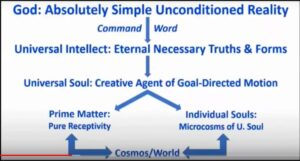
\includegraphics[scale=.6]{a20220824MeditationontheTrinity-img001.jpg}
 \end{wrapfigure}

God is the supreme person and is determined by nothing outside himself; otherwise, He would not be absolute. Yet, the Trinity follows from His nature, so in this sense the Trinity is necessary.

Here we can only provide a brief outline. For more detail, I can only recommend a close study of the three resources mentioned above. It is an important issue and well worth one's effort and time.



\flrightit{Posted on 2022-08-24 by Cologero }

\begin{center}* * *\end{center}

\begin{footnotesize}\begin{sffamily}



\texttt{Balder on 2022-08-29 at 14:02 said: }

@ArthurKonrad: about Guenon and his apparent lack of humor, he said in some of his writings something like following: ``it seems our writings are profoundly lacking joy, yet it is dependent on one's character what things give one the sense of joy."

So perhaps he was not humorless at all but found his joy elsewhere than from joking and common humor. I am a joker myself but I would find it quite strange if a book on metaphysics, symbolism or traditional sciences would be replete with jokes and humor.


\hfill

\texttt{Arthur Konrad on 2022-08-29 at 15:57 said: }

@Balder,

I won't discuss Guenon right now. I will however, make a general observation that there seems to be an entrenched antagonism between theologians and meta-physicians on one hand, and mystics on the other. Mystics (and here I'm using the common, broad meaning of it), being persons who typically do posses a sense of humour, are immunised against every sort of pretense, not in the least pretense to authority. The former camp responds very predictably, by accusing mystics of being `dangerous charlatans'. or using any similar tactic of discrediting a person by appealing to people's regard for their own safety and conformity.

Differences, as anyone with subtlety understands – presuming that he wants to – are not doctrinal, but a matter of personal animosity and vanity. Don't believe me? Just observe the rage that follows any real or perceived insult to the meta-physician's authority. All of a sudden, the wise man displays admirable skill in ad hominem attacks, punches under the belly and throws himself tooth and claw at the person's reputation and his right to decency. Then being `above dialectics' breaks like a pinata, and the onlookers can admire the fabulous fruits of a strictly meditative diet.

In such an environment one cannot learn much about the `Truth'. but he can learn quite a lot about politics, for instance. Science prevails elsewhere.


\hfill


\hfill

\texttt{Dionysus on 2023-05-15 at 22:03 said: }

Basically, the first objection the Greek partisans will make to the Filioque is that it's ``heresy". Such claim is absurd, since none of the Holy Fathers teaches against it explicitly, and many of them on the contrary clearly teach the Filioque, such as basically all the Latin Fathers, most notably Augustine, but also Greek Fathers such as Dydimus, Cyril of Alexandria and Maximus the Confessor. Such confusion could be explained by a quirk in translation, whereas in Greek the use of the word ``and" implicitly means that It proceeds equally from the Father and the Son, when in Latin it is ambiguous, meaning in this instance not equally but ``through", but that is another question (which is actually explaind by Saint Maximus). We could of course go into detail on the actual theological arguments, but that would be too much; I would like only to add to what was said in the text that, if the Spirit proceeded from the Father alone, its procession would be no different from the Son's generation, and the Spirit no different from the Son, not to mention that there is more than one biblical evidence for its procession through the Son, such as in the apocalyptic symbol of the River springing forth from the Lamb.

When the accusation of heresy is refuted, they will claim that it was illicit to change the text of the Creed, as it was prohibited by the Council Fathers of Nicaea I. Well, it is understood that such prohibition could only be against changes that would corrupt the deeper meaning of the Doctrine (that is, one that would teach heresy and not a change that would more clearly explain the true Faith), and not only a change in the letters themselves, otherwise it would be illicit to make any translations of the Creed, which is absurd.

Interestingly enough, the polemicist Photius (who was curiously only canonised by a Synod in Constantinople almost a thousand years after his death, with no prior public veneration, and at a point of heightened opposition of the Latin Church among the Orthodox) was the one who, trying to upset Rome, changed the words of the Creed and the meaning of the Doctrine by making it say ``from the Father alone/only" which was never thaught by any of the Holy Fathers (as even those who wrote only abouth the procession from the Father never said ``from the Father only" thus never deinying the possibility of the procession through the Son), which can both be classified as heresy and an adulteration of the text of the Creed in an unlawful way, also according to the Greek partisans own standards.

It is more than clear to me that such petty theological squables, as well as other meaningless polemics (such as the Greek partisans infatuation with leavened/unleavend bread, priestly marriage and use of beards), were never the cause or even major factors for the schism, but quite simply the refusal to recognise the authority and sovereignty of the Pope over the universal Church, an attitude that also has its roots in nothing more than historical factors regarding the growth of power of the See of Constantinople as the capital of the Eastern Empire and its defiance regarding the centralization of ecclesiastical power in Rome over the centuries, something that also explains why it was always Rome the one open to reunion while the Greeks were and still are always predominantly the ones fomenting petty divisions.


\end{sffamily}\end{footnotesize}
